%\documentclass[12pt,handout]{beamer}
\documentclass{beamer}
\usepackage[ngerman]{babel}
\usepackage[utf8]{inputenc}
\usepackage{amsmath}
\usepackage{amssymb}
\usepackage{listings} 
\usepackage{stmaryrd}
\lstset{language=Python, tabsize=4, basicstyle=\footnotesize, showstringspaces=false,mathescape=true}  
\usepackage{mathtools}
\usepackage{ulem}
\usepackage{tikz}

\usetheme{Boadilla}
\mode<presentation>{
\useoutertheme[subsection=false]{miniframes}
\useinnertheme{rectangles}
%\usecolortheme{crane}
}
\parskip 10pt



\begin{document}
\title{Informatik}   
\author{HeapSort} 
\date{}
\frame{\titlepage} 

%---

\begin{frame}[fragile]

\begin{tikzpicture}[level distance=10mm]
\tikzstyle{every node}=[draw,circle,inner sep=1pt]
\tikzstyle{level 1}=[sibling distance=30mm]

\tikzstyle{level 2}=[sibling distance=20mm]
\tikzstyle{level 3}=[sibling distance=10mm]
\node {~~~~}
child {node {~~~~}
child {node {~~~~}
}
child {node {~~~~}
}
}
child {node {~~~~}
child {node {~~~~}
}
child {node {~~~~}
child {node {~~~~}
}
child {node {~~~~}
}
}
};
\end{tikzpicture} 

Ein \textit{binärer Baum} ist entweder leer oder besteht aus einem Knoten, dem zwei binäre Bäume zugeordnet sind. \pause Dieser heißt dann \textit{Vater} des linken bzw. rechten Teilbaums. \pause Ein Knoten ohne Vater heißt \textit{Wurzel}. \pause Die Knoten, die x zum Vater haben, sind seine \textit{Söhne}. Knoten ohne Söhne heißen
 \textit{Blätter}. \pause

Im Beispiel hat der Baum 4 Ebenen. Die Wurzel ist auf Ebene 0, die zwei rechten Blätter sind auf Ebene 3.
\end{frame}

%---
\begin{frame}[fragile]
Ein \textit{Heap} ist ein binärer Baum für den gilt:  
\begin{itemize}
\item Jeder Knoten enthält einen Schlüssel \\ \pause
\item Schlüssel im Vater $\le$ Schlüssel im Sohn \\ \pause 
\item Alle Ebenen sind vollständig gefüllt, bis auf die letzte, die muss von links beginnend gefüllt sein. \pause
\end{itemize}

Die Umrisse eines Heaps: 

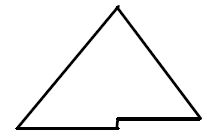
\includegraphics[scale=0.6]{heap.png}
\end{frame}

%---
\begin{frame}[fragile]
Ein Heap 

\begin{tikzpicture}[level distance=10mm]
\tikzstyle{every node}=[draw,circle,inner sep=1pt]
\tikzstyle{level 1}=[sibling distance=30mm]

\tikzstyle{level 2}=[sibling distance=20mm]
\tikzstyle{level 3}=[sibling distance=10mm]
\node {42}
child {node {80}
child {node {90}
child {node {92}}
child {node {94}}
}
child {node {81}
child {node {93}}
child {node {90}}
}
}
child {node {55}
child {node {60}}
child {node {58}}
};
\end{tikzpicture} \pause 

\begin{tabular}{llllllllllllllllllll}
& 42 & 80 & 55 & 90 & 81 & 60 & 58 & 92 & 94 & 93 & 90 \\
Index: & 0 & 1 & 2 & 3 & 4 & 5 & 6 & 7 & 8 & 9 & 10
\end{tabular}

linker Sohn von Knoten i: ~~~\pause 2i+1  \\
rechter Sohn von Knoten i:  ~\pause 2i+2  \\
Vater von Knoten i: ~~~~~~~~~ \pause (i$-$1)//2

\end{frame}

%---
\begin{frame}[fragile]
Idee für HeapSort: 

Gegeben Liste $[a_0, a_1, ... , a_{n-1}]$ \\ 
Konstruiere daraus einen Heap. \\ 
for i in range(n):\\  
~~~~ liefere Wurzel als aktuelles Minimum; \\  
~~~~ entferne Wurzel; \\ 
~~~~ reorganisiere Heap; \\


\end{frame}

%----
\begin{frame}[fragile]
\begin{minipage}{5.5cm}
\begin{tikzpicture}[level distance=10mm]
\tikzstyle{every node}=[draw,circle,inner sep=1pt]
\tikzstyle{level 1}=[sibling distance=25mm]

\tikzstyle{level 2}=[sibling distance=15mm]
\tikzstyle{level 3}=[sibling distance=10mm]
\node {42}
child {node {50}
child {node {61}
child {node {70}}
child {node {72}}}
child {node {65}
child {node {78}}
}
}
child {node {70}
child {node {81}}
child {node {82}}
}
;
\end{tikzpicture} 
\end{minipage}
\begin{minipage}{5.5cm}
\begin{tikzpicture}[level distance=10mm]
\tikzstyle{every node}=[draw,circle,inner sep=1pt]
\tikzstyle{level 1}=[sibling distance=25mm]

\tikzstyle{level 2}=[sibling distance=15mm]
\tikzstyle{level 3}=[sibling distance=10mm]
\node {~~~~}
child {node {50}
child {node {61}
child {node {70}}
child {node {72}}}
child {node {65}
child {node {78}}
}
}
child {node {70}
child {node {81}}
child {node {82}}
}
;
\end{tikzpicture} 
\end{minipage}

\hspace{5.5cm}42
\end{frame}


%----
\begin{frame}[fragile]


\begin{minipage}{5.5cm}
\begin{tikzpicture}[level distance=10mm]
\tikzstyle{every node}=[draw,circle,inner sep=1pt]
\tikzstyle{level 1}=[sibling distance=25mm]

\tikzstyle{level 2}=[sibling distance=15mm]
\tikzstyle{level 3}=[sibling distance=10mm]


\node {50}
child {node {61}
child {node {70}
child {node {78}}
child {node {72}}}
child {node {65}
}
}
child {node {70}
child {node {81}}
child {node {82}}
}
;
\end{tikzpicture} 
\end{minipage}

\hspace{5.5cm}Das Ergebnis ist ein Heap
\end{frame}

%---
\begin{frame}[fragile]
Aufwand für Reorganisation 

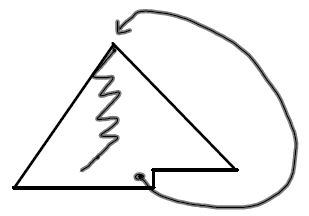
\includegraphics[scale=0.6]{heap2.png}

proportional zur Länge des Wegs: \pause $O(\log n)$
\end{frame}

%---
\begin{frame}[fragile]

\begin{minipage}[c]{7cm}
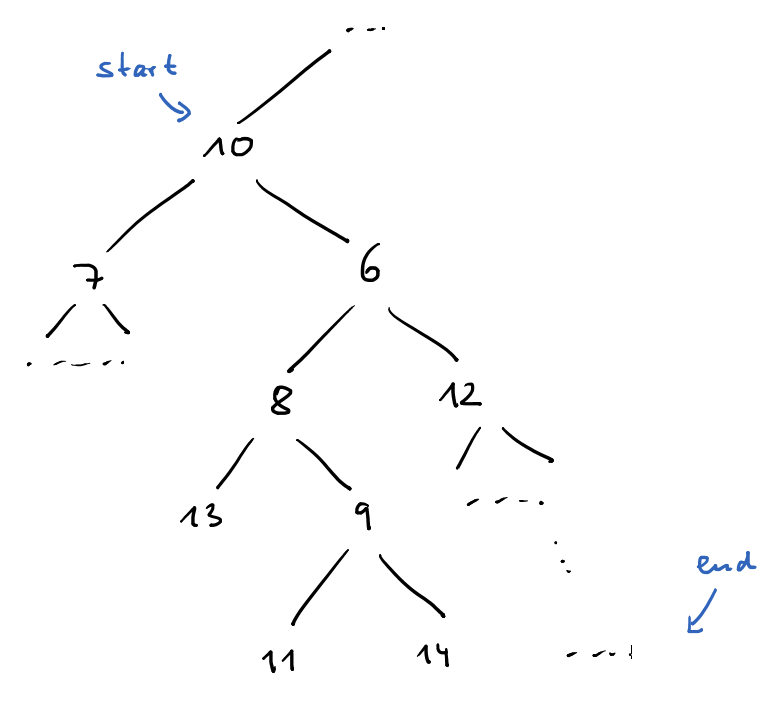
\includegraphics[width=7cm]{heap4.png}
\end{minipage}
\begin{minipage}[c]{4cm}
Die Funktion \texttt{sift} prüft, ob zwischen \texttt{start} und \texttt{end} ein ordentlicher Heap ist, oder ob \texttt{start} versickern muss.
Die Funktion kann sich darauf verlassen, dass unterhalb von \texttt{start} alles in Ordnung ist.
\end{minipage}
\end{frame}

%---
\begin{frame}[fragile]

\begin{lstlisting} 
def sift(a, start , end):
    i = start
    x = a[start]
    j = 2 * i + 1
    if j < end and a[j+1] < a[j]:
        j+=1
    while j <= end and a[j] < x:
        a[i] = a[j]
        i = j
        j = j * 2 + 1
        if j < end and a[j+1] < a[j]:
            j+=1
    a[i] = x
\end{lstlisting} 
\end{frame}

%---
\begin{frame}[fragile]
Aufbau eines Heaps  

Gegeben Liste a:  14 42 2 13 7 24 49 5 18 \\
Schreibe die Liste als Baum  

\begin{tikzpicture}[level distance=10mm]
\tikzstyle{every node}=[draw,circle,inner sep=1pt]
\tikzstyle{level 1}=[sibling distance=25mm]
\tikzstyle{level 2}=[sibling distance=15mm]
\tikzstyle{level 3}=[sibling distance=7mm]
\node {14}
child {node {42}
child {node {13}
child {node {5}}
child {node {18}}
}
child {node {7}
}
}
child {node {2}
child {node {24}}
child {node {49}}
};
\end{tikzpicture} \pause 


letzter Knoten: ~~~~~\pause a[len(a)-1] \\ \pause 
Vater des letzten Knotens: \pause a[(len(a)-2)//2] \pause 

Beginne beim Vater des letzten Knotens. Gehe von dort rückwärts Ebene für Ebene durch und rufe den Elementen jeweils \textit{sift} zu.
\end{frame}

\begin{frame}[fragile]

\begin{tikzpicture}[level distance=10mm]
\tikzstyle{every node}=[draw,circle, text width=0.4cm,inner sep=1pt]
%\tikzstyle{every node}=[draw,circle(1),inner sep=1pt]
\tikzstyle{level 1}=[sibling distance=25mm]
\tikzstyle{level 2}=[sibling distance=15mm]
\tikzstyle{level 3}=[sibling distance=7mm]



\node {2}
child {node {5}
child {node {13}
child {node {42}}
child {node {18}}
}
child {node {7}
}
}
child {node {14}
child {node {24}}
child {node {49}}
};

\end{tikzpicture} 

Die Liste nach Aufbau des Heaps:

2 5 14 13 7 24 49 42 18
\end{frame}

 
\begin{frame}[fragile]
Inhalt der Liste nach jeder Reorganisation:

2 5 14 13 7 24 49 42 18 \\
5 7 14 13 18 24 49 42 \alert{2} \\
7 13 14 42 18 24 49 \alert{5 2} \\
13 18 14 42 49 24  \alert{7 5 2} \\
14 18 24 42 49 \alert{13 7 5 2 \\}
18 42 24 49 \alert{14 13 7 5 2 \\}
24 42 49 \alert{18 14 13 7 5 2 \\}
42 49 \alert{24 18 14 13 7 5 2 \\}
49 \alert{42 24 18 14 13 7 5 2 \\}

\end{frame}

%------
\begin{frame}[fragile]

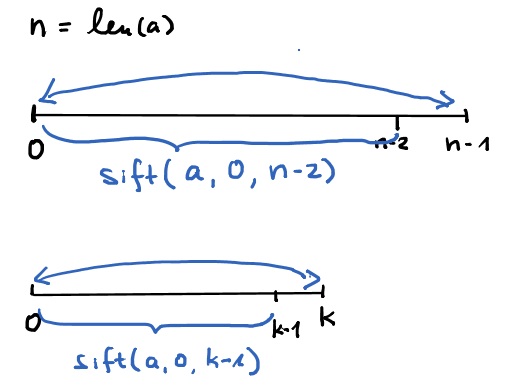
\includegraphics[scale=0.5]{heap5.png} \pause

\begin{lstlisting} 
def heap_sort(a):
    n = len(a)
    for k in range ((n-2)//2,-1,-1):
        sift(a,k,n-1)
    for k in range(n-1,0,-1):
        a[0],a[k]=a[k],a[0]
        sift(a,0,k-1)
\end{lstlisting} 
\end{frame}


%------
\begin{frame}[fragile]

Analyse von HeapSort 

Aufwand für Aufbau des Heaps: \pause $O(n)$  \\  
(Ca. die Hälfte der Elemente des Heaps sind Blätter, nur jeweils ca. n/2 Elemente müssen reorganisiert werden, 
wobei - nach oben hin - die Anzahl de  Elemente mit den längeren Sickerwegen abnimmt.)   

Aufwand für eine Reorganisation:  \pause  $O(\log n)$

Insgesamt: $O(n \cdot \log n)$ im best, worst und average case.  

Zusätzlicher Platzbedarf:  \pause  $O(1)$

\end{frame}


%------
\begin{frame}[fragile]

Laufzeit und Platzbedarf der Sortieralgorithmen  

\footnotesize
\begin{tabular}{| l | l | l | l | l |}
\hline
& best   &   average & worst & zusätzlicher Platz \\ 
\hline
SelectionSort & \uncover<3->{$O(n^2)}$ & \uncover<3->{$O(n^2)$} & \uncover<3->{$O(n^2)$} &  \uncover<4->{$O(1)$} \\
\hline
BubbleSort & \uncover<5->{$O(n)$} & \uncover<5->{$O(n^2)$} & \uncover<5->{$O(n^2)$} &  \uncover<6->{$O(1)$} \\
\hline
MergeSort &  \uncover<7->{$O(n \cdot \log n)$}  & \uncover<7->{$O(n \cdot \log n)$} & \uncover<7->{$O(n \cdot \log n)$}  &  \uncover<8->{$O(n)$} \\
\hline
QuickSort &  \uncover<9->{$O(n \cdot \log n)$}  & \uncover<9->{$O(n \cdot \log n)$} & \uncover<9->{$O(n^2)$} &  \uncover<10->{$O(\log n)$} \\
\hline
HeapSort &  \uncover<11->{$O(n \cdot \log n)$}  & \uncover<11->{$O(n \cdot \log n)$} & \uncover<11->{$O(n \cdot \log n)$} &  \uncover<12->{$O(1)$}  \\
\hline
\end{tabular}

\end{frame}
 \end{document}